\documentclass[12pt, titlepage]{article}

\usepackage{fullpage}
\usepackage[round]{natbib}
\usepackage{multirow}
\usepackage{booktabs}
\usepackage{tabularx}
\usepackage{graphicx}
\usepackage{float}
\usepackage{hyperref}
\hypersetup{
    colorlinks,
    citecolor=blue,
    filecolor=black,
    linkcolor=red,
    urlcolor=blue
}

%% Comments

\usepackage{color}

\newif\ifcomments\commentstrue %displays comments
%\newif\ifcomments\commentsfalse %so that comments do not display

\ifcomments
\newcommand{\authornote}[3]{\textcolor{#1}{[#3 ---#2]}}
\newcommand{\todo}[1]{\textcolor{red}{[TODO: #1]}}
\else
\newcommand{\authornote}[3]{}
\newcommand{\todo}[1]{}
\fi

\newcommand{\wss}[1]{\authornote{blue}{SS}{#1}} 
\newcommand{\plt}[1]{\authornote{magenta}{TPLT}{#1}} %For explanation of the template
\newcommand{\an}[1]{\authornote{cyan}{Author}{#1}}

%% Common Parts

\newcommand{\progname}{ProgName} % PUT YOUR PROGRAM NAME HERE
\newcommand{\authname}{Team \#, Team Name
\\ Student 1 name
\\ Student 2 name
\\ Student 3 name
\\ Student 4 name} % AUTHOR NAMES                  

\usepackage{hyperref}
    \hypersetup{colorlinks=true, linkcolor=blue, citecolor=blue, filecolor=blue,
                urlcolor=blue, unicode=false}
    \urlstyle{same}
                                


\newcounter{acnum}
\newcommand{\actheacnum}{AC\theacnum}
\newcommand{\acref}[1]{AC\ref{#1}}

\newcounter{ucnum}
\newcommand{\uctheucnum}{UC\theucnum}
\newcommand{\uref}[1]{UC\ref{#1}}

\newcounter{mnum}
\newcommand{\mthemnum}{M\themnum}
\newcommand{\mref}[1]{M\ref{#1}}

\begin{document}

\title{Module Guide for \progname{}} 
\author{\authname}
\date{\today}

\maketitle

\pagenumbering{roman}

\section{Revision History}

\begin{tabularx}{\textwidth}{p{3cm}p{2cm}X}
\toprule {\bf Date} & {\bf Version} & {\bf Notes}\\
\midrule
January 13, 2025 & 1.0 & Initial Revision\\
January 17, 2025 & 1.1 & Final changes made according to rubric\\
\bottomrule
\end{tabularx}

\newpage

\section{Reference Material}

This section records information for easy reference. 

\subsection{Abbreviations and Acronyms}

\renewcommand{\arraystretch}{1.2}
\begin{tabular}{l l} 
  \toprule		
  \textbf{symbol} & \textbf{description}\\
  \midrule 
  AC & Anticipated Change\\
  DAG & Directed Acyclic Graph \\
  M & Module \\
  MG & Module Guide \\
  OS & Operating System \\
  R & Requirement\\
  SC & Scientific Computing \\
  SRS & Software Requirements Specification\\
  \progname & Explanation of program name\\
  UC & Unlikely Change \\
  \wss{etc.} & \wss{...}\\
  \bottomrule
\end{tabular}\\

\newpage

\tableofcontents

\listoftables

\listoffigures

\newpage

\pagenumbering{arabic}

\section{Introduction}

Decomposing a system into modules is a commonly accepted approach to developing
software.  A module is a work assignment for a programmer or programming
team~\citep{ParnasEtAl1984}.  We advocate a decomposition
based on the principle of information hiding~\citep{Parnas1972a}.  This
principle supports design for change, because the ``secrets'' that each module
hides represent likely future changes.  Design for change is valuable in SC,
where modifications are frequent, especially during initial development as the
solution space is explored.  

Our design follows the rules layed out by \citet{ParnasEtAl1984}, as follows:
\begin{itemize}
\item System details that are likely to change independently should be the
  secrets of separate modules.
\item Each data structure is implemented in only one module.
\item Any other program that requires information stored in a module's data
  structures must obtain it by calling access programs belonging to that module.
\end{itemize}

After completing the first stage of the design, the Software Requirements
Specification (SRS), the Module Guide (MG) is developed~\citep{ParnasEtAl1984}. The MG
specifies the modular structure of the system and is intended to allow both
designers and maintainers to easily identify the parts of the software.  The
potential readers of this document are as follows:

\begin{itemize}
\item New project members: This document can be a guide for a new project member
  to easily understand the overall structure and quickly find the
  relevant modules they are searching for.
\item Maintainers: The hierarchical structure of the module guide improves the
  maintainers' understanding when they need to make changes to the system. It is
  important for a maintainer to update the relevant sections of the document
  after changes have been made.
\item Designers: Once the module guide has been written, it can be used to
  check for consistency, feasibility, and flexibility. Designers can verify the
  system in various ways, such as consistency among modules, feasibility of the
  decomposition, and flexibility of the design.
\end{itemize}

The rest of the document is organized as follows. Section
\ref{SecChange} lists the anticipated and unlikely changes of the software
requirements. Section \ref{SecMH} summarizes the module decomposition that
was constructed according to the likely changes. Section \ref{SecConnection}
specifies the connections between the software requirements and the
modules. Section \ref{SecMD} gives a detailed description of the
modules. Section \ref{SecTM} includes two traceability matrices. One checks
the completeness of the design against the requirements provided in the SRS. The
other shows the relation between anticipated changes and the modules. Section
\ref{SecUse} describes the use relation between modules.

\section{Anticipated and Unlikely Changes} \label{SecChange}

This section lists possible changes to the system. According to the likeliness
of the change, the possible changes are classified into two
categories. Anticipated changes are listed in Section \ref{SecAchange}, and
unlikely changes are listed in Section \ref{SecUchange}.

\subsection{Anticipated Changes} \label{SecAchange}

Anticipated changes are the source of the information that is to be hidden
inside the modules. Ideally, changing one of the anticipated changes will only
require changing the one module that hides the associated decision. The approach
adapted here is called design for
change.

\begin{description}
\item[\refstepcounter{acnum} \actheacnum \label{ac1}:] Supporting additional hardware, such as new touchscreen displays or tablets, to ensure compatibility with future device upgrades and varying specifications.
\item[\refstepcounter{acnum} \actheacnum \label{ac2}:] Modifying input data formats to align with updated composite structures or metadata provided by Lifetouch.
\item [\refstepcounter{acnum} \actheacnum \label{ac3}:] Enhancing data processing workflows to adapt to different composite formats and improve OCR preprocessing accuracy.
  \item [\refstepcounter{acnum} \actheacnum \label{ac4}:] Scaling the system to include graduation composites from additional faculties or departments across the university.
  \item [\refstepcounter{acnum} \actheacnum \label{ac5}:] Updating the OCR model to accommodate higher-resolution composites or address accuracy improvements in text extraction.
  \item [\refstepcounter{acnum} \actheacnum \label{ac6}:] Adding new user roles, such as external recruiters or event organizers, to expand the system's usability and access controls.
  \item [\refstepcounter{acnum} \actheacnum \label{ac7}:] Redesigning the user interface to meet evolving accessibility standards and usability feedback for a better experience.
  \item [\refstepcounter{acnum} \actheacnum \label{ac8}:] Extending the database schema to store new metadata, such as additional student achievements or career milestones.
  \item [\refstepcounter{acnum} \actheacnum \label{ac9}:] Integrating the system with McMaster’s existing alumni and event management platforms to streamline user engagement.
  \item [\refstepcounter{acnum} \actheacnum \label{ac10}:] Adjusting backend processes to comply with updates to privacy policies, legal regulations, or internal university standards.
\end{description}

\wss{Anticipated changes relate to changes that would be made in requirements,
design or implementation choices.  They are not related to changes that are made
at run-time, like the values of parameters.}

\subsection{Unlikely Changes} \label{SecUchange}

The module design should be as general as possible. However, a general system is
more complex. Sometimes this complexity is not necessary. Fixing some design
decisions at the system architecture stage can simplify the software design. If
these decision should later need to be changed, then many parts of the design
will potentially need to be modified. Hence, it is not intended that these
decisions will be changed.

\begin{description}
\item[\refstepcounter{ucnum} \uctheucnum \label{ucIO}:] The source of the input data will always be from predefined repositories, such as LifeTouch or McMaster databases.
\item[\refstepcounter{ucnum} \uctheucnum \label{ucIO}:] The system will always display graduation composites on touchscreen interfaces and other devices as defined during development.
  \item[\refstepcounter{ucnum} \uctheucnum \label{ucIO}:] The primary goal of the system will remain focused on facilitating the browsing and searching of graduation composites for students, alumni, and staff.
  \item[\refstepcounter{ucnum} \uctheucnum \label{ucIO}:] The search functionality will always rely on a combination of Optical Character Recognition (OCR) data and metadata stored within the system.
  \item[\refstepcounter{ucnum} \uctheucnum \label{ucIO}:] The backend database architecture will remain relational (or NoSQL, as selected initially) to meet system scalability and storage requirements.
  \item[\refstepcounter{ucnum} \uctheucnum \label{ucIO}:] The system will only support English as the primary language for search and display functionalities.
  \item[\refstepcounter{ucnum} \uctheucnum \label{ucIO}:] The project will be exclusively deployed on McMaster’s internal infrastructure, adhering to university IT policies and avoiding external hosting solutions.
  \item[\refstepcounter{ucnum} \uctheucnum \label{ucIO}:] The privacy and security protocols implemented will always follow GDPR and university policies, ensuring compliance with data handling standards.
\end{description}

\section{Module Hierarchy} \label{SecMH}

This section provides an overview of the module design. Modules are summarized
in a hierarchy decomposed by secrets in Table \ref{TblMH}. The modules listed
below, which are leaves in the hierarchy tree, are the modules that will
actually be implemented.

\begin{description}
\item [\refstepcounter{mnum} \mthemnum \label{mHH}:] Cloud
\item [\refstepcounter{mnum} \mthemnum \label{mIF}:] Input Format
\item [\refstepcounter{mnum} \mthemnum \label{mDU}:] Data Upload
\item [\refstepcounter{mnum} \mthemnum \label{mOCRP}:] OCR Processing
\item [\refstepcounter{mnum} \mthemnum \label{mOS}:] Output Storage
\item [\refstepcounter{mnum} \mthemnum \label{mUIP}:] UI Parsing
\item [\refstepcounter{mnum} \mthemnum \label{mGUI}:] Graphical User Interface
\end{description}


\begin{table}[h!]
\centering
\begin{tabular}{p{0.3\textwidth} p{0.6\textwidth}}
\toprule
\textbf{Level 1} & \textbf{Level 2}\\
\midrule

{Hardware-Hiding Module} & Cloud \\
\midrule

\multirow{7}{0.3\textwidth}{Behaviour-Hiding Module} & Input Format\\
& Data Upload\\
& OCR Processing\\
& Output Storage\\
\midrule

\multirow{3}{0.3\textwidth}{Software Decision Module} & {UI Parsing}\\
& Graphical User Interface\\
\bottomrule

\end{tabular}
\caption{Module Hierarchy}
\label{TblMH}
\end{table}

\section{Connection Between Requirements and Design} \label{SecConnection}

The design of the system is intended to satisfy the requirements developed in
the SRS. In this stage, the system is decomposed into modules. The connection
between requirements and modules is listed in Table~\ref{TblRT}.

\wss{The intention of this section is to document decisions that are made
  ``between'' the requirements and the design.  To satisfy some requirements,
  design decisions need to be made.  Rather than make these decisions implicit,
  they are explicitly recorded here.  For instance, if a program has security
  requirements, a specific design decision may be made to satisfy those
  requirements with a password.}

\section{Module Decomposition} \label{SecMD}

Modules are decomposed according to the principle of ``information hiding''
proposed by \citet{ParnasEtAl1984}. The \emph{Secrets} field in a module
decomposition is a brief statement of the design decision hidden by the
module. The \emph{Services} field specifies \emph{what} the module will do
without documenting \emph{how} to do it. For each module, a suggestion for the
implementing software is given under the \emph{Implemented By} title. If the
entry is \emph{OS}, this means that the module is provided by the operating
system or by standard programming language libraries.  \emph{\progname{}} means the
module will be implemented by the \progname{} software.

Only the leaf modules in the hierarchy have to be implemented. If a dash
(\emph{--}) is shown, this means that the module is not a leaf and will not have
to be implemented.

\subsection{Hardware Hiding Modules}

\begin{description}
\item[Secrets:]The data structure and algorithm used to implement the virtual
  hardware.
\item[Services:]Serves as a virtual hardware used by the rest of the
  system. This module provides the interface between the hardware and the
  software. So, the system can use it to display outputs or to accept inputs.
\item[Implemented By:] OS
\end{description}

\subsubsection{Cloud Module (\mref{mHH})}

\begin{description}
\item[Secrets:]The SDKs, APIs, and configurations used to interact with AWS (S3, Lambda, and DynamoDB), including details of network protocols, security settings, and hardware infrastructure.
\item[Services:]Provides a virtual hardware layer by abstracting cloud storage (Amazon S3), serverless compute (AWS Lambda), and database operations (Amazon DynamoDB). Allows the system to upload and retrieve data, execute image processing logic, and store processed metadata seamlessly without exposing hardware details.
\item[Implemented By:] AWS Services and SDKs
\item[Type of Module:] Abstract Object
\end{description}

\subsection{Behaviour-Hiding Module}

\begin{description}
\item[Secrets:]The contents of the required behaviours.
\item[Services:]Includes programs that provide externally visible behaviour of
  the system as specified in the software requirements specification (SRS)
  documents. This module serves as a communication layer between the
  hardware-hiding module and the software decision module. The programs in this
  module will need to change if there are changes in the SRS.
\item[Implemented By:] --
\end{description}

\subsubsection{Input Module (\mref{mIF})}

\begin{description}
\item[Secrets:]The structure of the image and metadata provided by the client (admin). Includes details such as accepted file formats, metadata keys, and expected payload structure.
\item[Services:]Converts client-provided data (composite image) into a format suitable for uploading to S3 and processing by Lambda. Ensures compliance with predefined input standards.
\item[Implemented By:] Back-End Entity
\item[Type of Module:] Library
\end{description}

\subsubsection{Data Upload Module (\mref{mDU})}

\begin{description}
\item[Secrets:]The configuration of API endpoints, security mechanisms (e.g., HTTPS, authentication), and retry logic for uploads.
\item[Services:]Handles the transfer of input data (image) to Amazon S3. Encapsulates the logic for SDK interactions, upload retries, and error handling.
\item[Implemented By:] Back-End Entity and AWS S3 Entity
\item[Type of Module:] Abstract Object
\end{description}

\subsubsection{OCR Processing Module (\mref{mOCRP})}

\begin{description}
\item[Secrets:]The OCR algorithm and processing logic for extracting names and center points of individuals from composite images.
\item[Services:]Processes the uploaded images to extract required metadata (e.g., individual names and center points). Transforms the processed data into a format ready for storage in DynamoDB.
\item[Implemented By:] AWS Lambda
\item[Type of Module:] Library
\end{description}

\subsubsection{Output Storage Module (\mref{mOS})}

\begin{description}
\item[Secrets:]The schema for DynamoDB, including primary keys, data types, and indexing strategies.
\item[Services:]Stores extracted data and metadata in DynamoDB for later retrieval. Abstracts database operations such as creating, reading, updating, and deleting records.
\item[Implemented By:] DynamoDB Entity
\item[Type of Module:] Abstract Data Type
\end{description}

\subsection{Software Decision Module}

\begin{description}
\item[Secrets:] The design decision based on mathematical theorems, physical
  facts, or programming considerations. The secrets of this module are
  \emph{not} described in the SRS.
\item[Services:] Includes data structure and algorithms used in the system that
  do not provide direct interaction with the user. 
  % Changes in these modules are more likely to be motivated by a desire to
  % improve performance than by externally imposed changes.
\item[Implemented By:] --
\end{description}

\subsubsection{UI Parsing Module (\mref{mUIP})}

\begin{description}
\item[Secrets:]The implementation logic for uploading images and viewing composite images through user interface and interactions.
\item[Services:]Implements rules for managing workflows, such as fallback mechanisms for failed uploads or processing. Encodes data transformation rules for formatting outputs.
\item[Implemented By:] Back-End Logic and AWS Lambda
\item[Type of Module:] Library
\end{description}

\subsubsection{Graphical User Interface Module (\mref{mGUI})}

\begin{description}
\item[Secrets:]User interaction event handling, user input controls, states, The methods to imple- ment data formats (such as text-boxes, buttons, file dialogs), visual layout and styling (eg. colours or sizing) for user interaction.
\item[Services:]Provides methods for building a visual interface for the user to see and interact with.
\item[Implemented By:] React
\item[Type of Module:] Library
\end{description}


\section{Traceability Matrix} \label{SecTM}

This section shows two traceability matrices: between the modules and the
requirements and between the modules and the anticipated changes.

% the table should use mref, the requirements should be named, use something
% like fref
\begin{table}[H]
\centering
\begin{tabular}{p{0.2\textwidth} p{0.6\textwidth}}
\toprule
\textbf{Req.} & \textbf{Modules}\\
\midrule
R1 & \mref{mIF}, \mref{mDU}, \mref{mUIP}, \mref{mGUI}\\
R2 & \mref{mHH}, \mref{mIF}, \mref{mDU}, \mref{mOCRP}, \mref{mOS}, \mref{mUIP}\\
R3 & \mref{mIF}, \mref{mGUI}\\
R4 & \mref{mOS}, \mref{mGUI}\\
R5 & \mref{mHH}, \mref{mOS}, \mref{mGUI}\\
R6 & \mref{mHH}, \mref{mIF}\\

\bottomrule
\end{tabular}
\caption{Trace Between Requirements and Modules}
\label{TblRT}
\end{table}

\begin{table}[H]
\centering
\begin{tabular}{p{0.2\textwidth} p{0.6\textwidth}}
\toprule
\textbf{AC} & \textbf{Modules}\\
\midrule
\acref{ac1} & \mref{mGUI}\\
\acref{ac2} & \mref{mIF}\\
\acref{ac3} & \mref{mOCRP}\\
\acref{ac4} & \mref{mHH}, \mref{mOS}\\
\acref{ac5} & \mref{mOCRP}\\
\acref{ac6} & \mref{mIF}, \mref{mGUI}\\
\acref{ac7} & \mref{mGUI}\\
\acref{ac8} & \mref{mOS}\\
\acref{ac9} & \mref{mHH}\\
\acref{ac10} & \mref{mHH}, \mref{mIF}\\
\bottomrule
\end{tabular}
\caption{Trace Between Anticipated Changes and Modules}
\label{TblACT}
\end{table}

\section{Use Hierarchy Between Modules} \label{SecUse}

In this section, the uses hierarchy between modules is
provided. \citet{Parnas1978} said of two programs A and B that A {\em uses} B if
correct execution of B may be necessary for A to complete the task described in
its specification. That is, A {\em uses} B if there exist situations in which
the correct functioning of A depends upon the availability of a correct
implementation of B.  Figure \ref{FigUH} illustrates the use relation between
the modules. It can be seen that the graph is a directed acyclic graph
(DAG). Each level of the hierarchy offers a testable and usable subset of the
system, and modules in the higher level of the hierarchy are essentially simpler
because they use modules from the lower levels.

\wss{The uses relation is not a data flow diagram.  In the code there will often
be an import statement in module A when it directly uses module B.  Module B
provides the services that module A needs.  The code for module A needs to be
able to see these services (hence the import statement).  Since the uses
relation is transitive, there is a use relation without an import, but the
arrows in the diagram typically correspond to the presence of import statement.}

\wss{If module A uses module B, the arrow is directed from A to B.}

\begin{figure}[H]
\centering
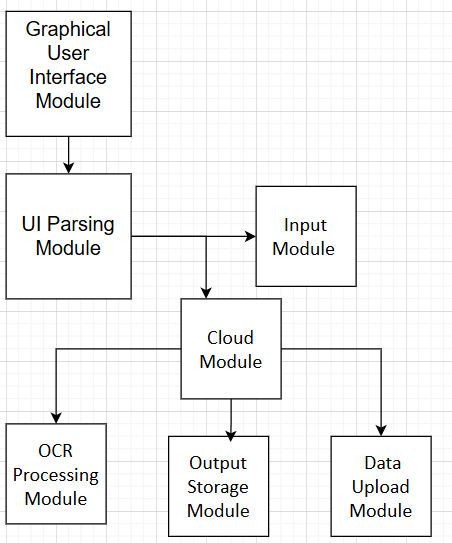
\includegraphics[width=0.7\textwidth]{image.png}
\caption{Use hierarchy among modules}
\label{FigUH}
\end{figure}

%\section*{References}

\section{User Interfaces}

\wss{Design of user interface for software and hardware.  Attach an appendix if
needed. Drawings, Sketches, Figma}

\begin{figure}[H]
\centering
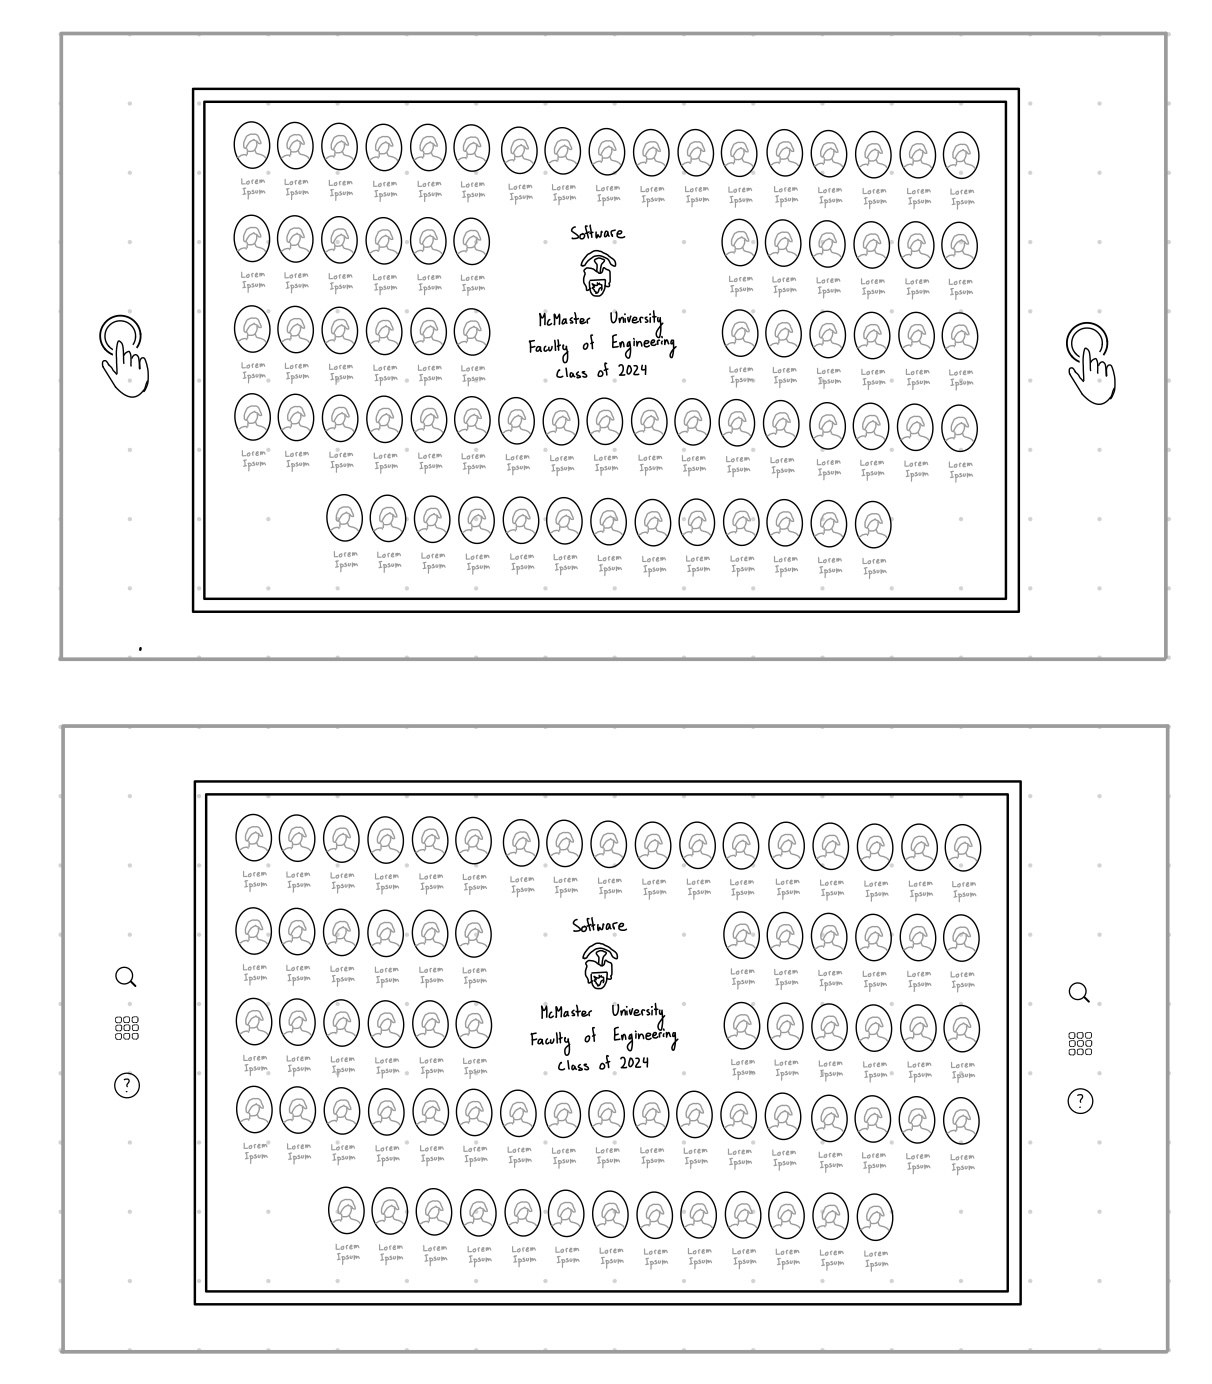
\includegraphics[width=0.7\textwidth]{IMG_0067.png}
\caption{User Interface Design}
\label{FigUH}
\end{figure}

\begin{figure}[H]
\centering
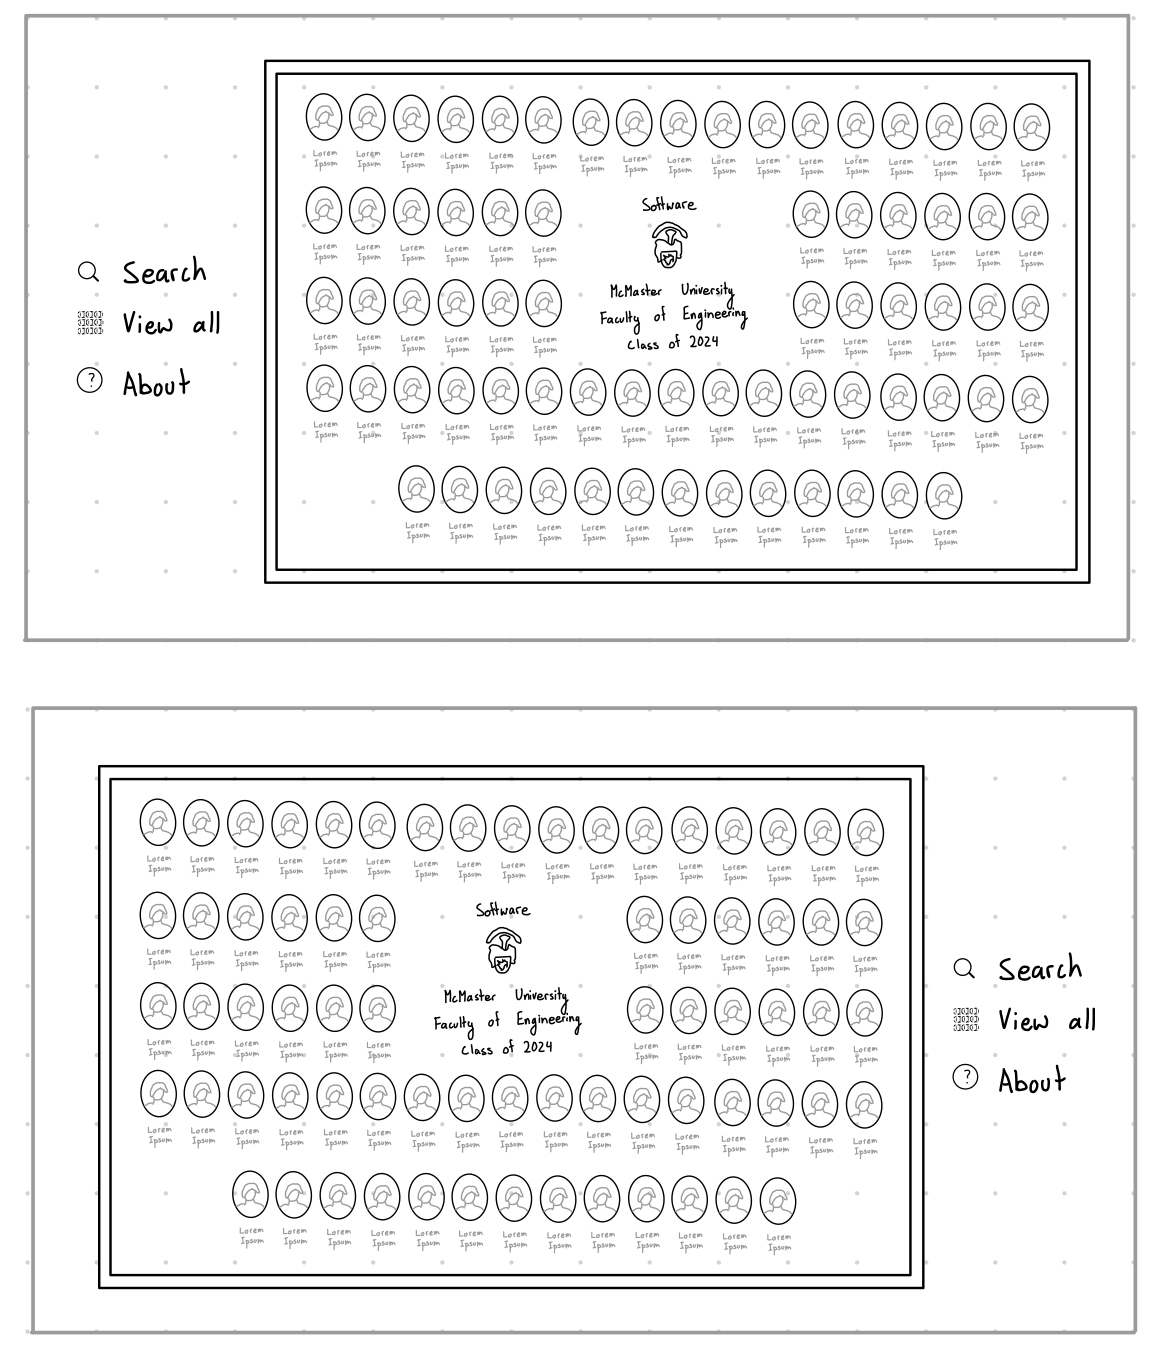
\includegraphics[width=0.7\textwidth]{IMG_0069.png}
\caption{User Interface Design}
\label{FigUH}
\end{figure}

\begin{figure}[H]
\centering
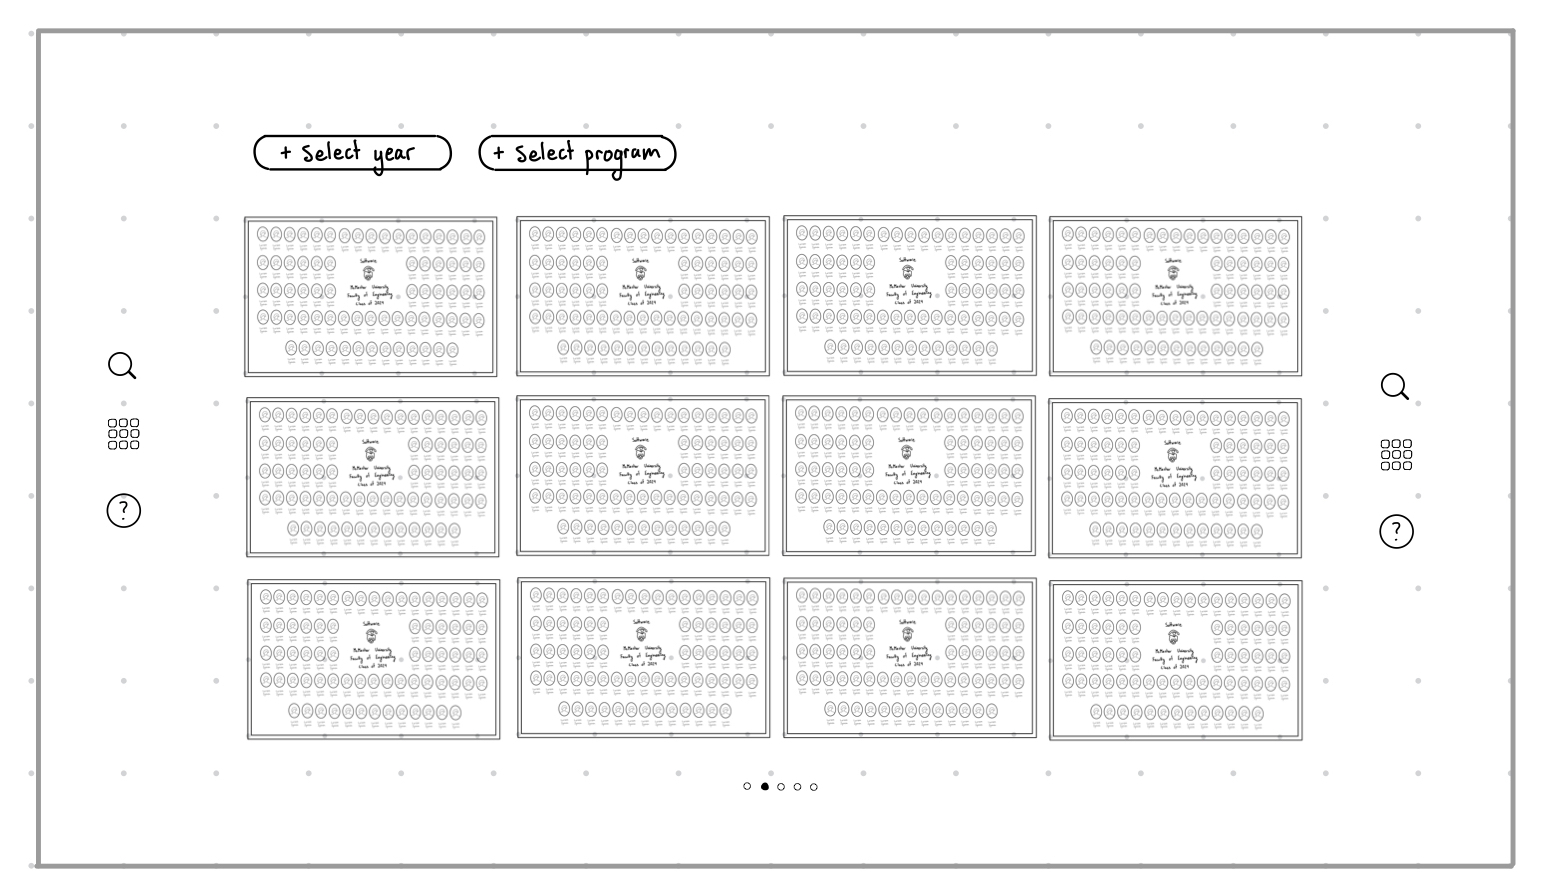
\includegraphics[width=0.7\textwidth]{IMG_0070.png}
\caption{User Interface Design}
\label{FigUH}
\end{figure}

\begin{figure}[H]
\centering
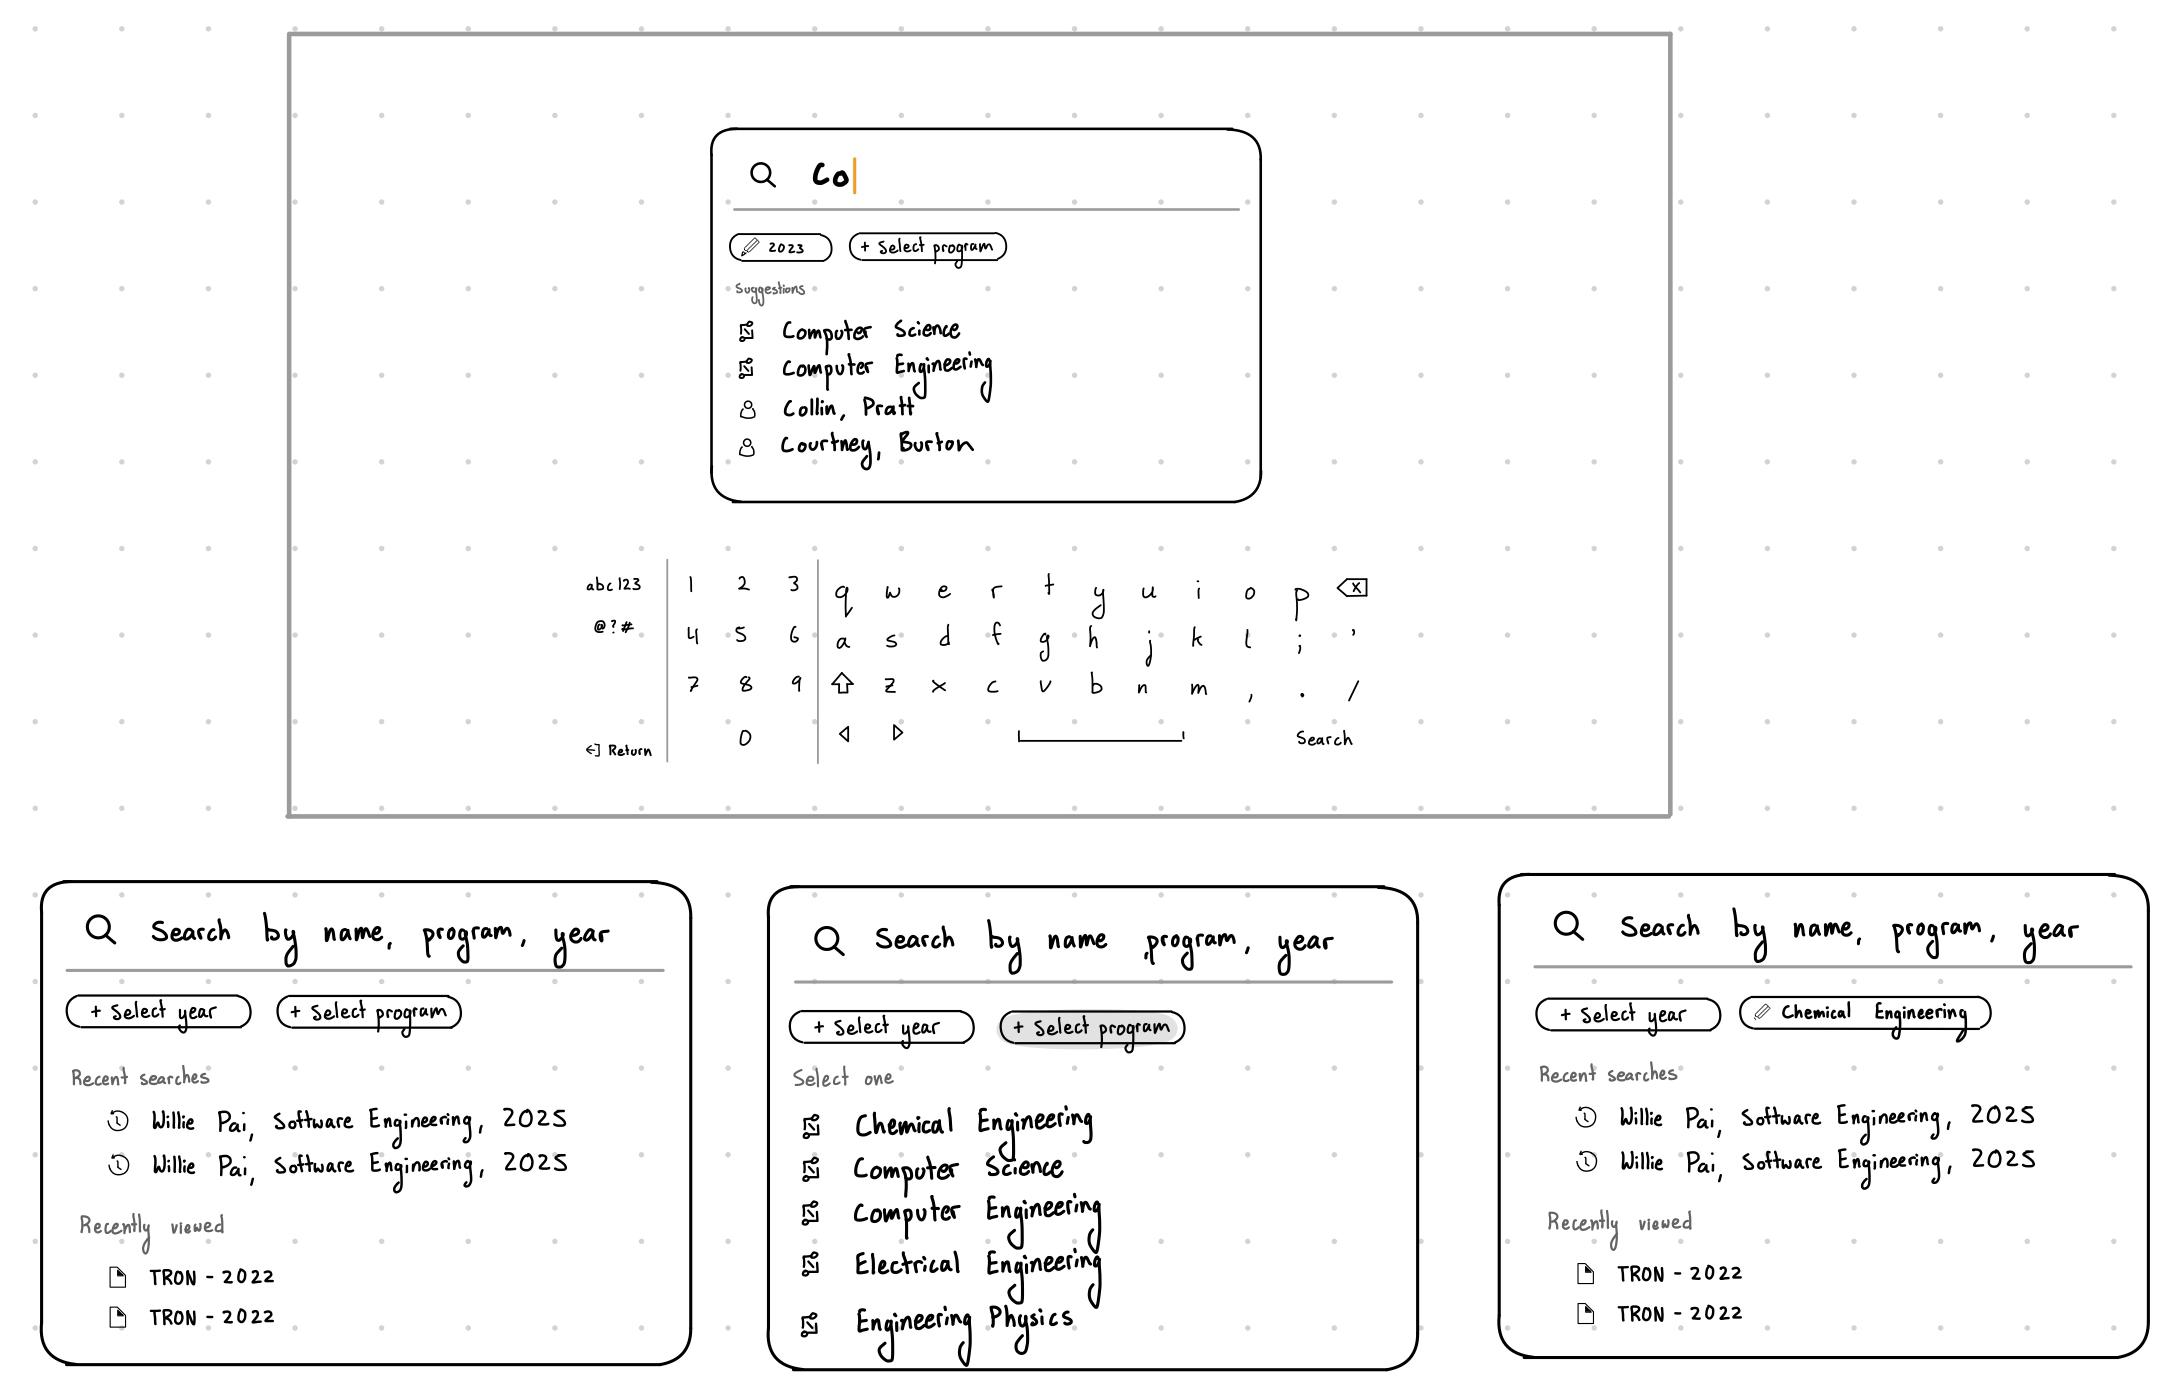
\includegraphics[width=0.7\textwidth]{IMG_0071.png}
\caption{User Interface Design}
\label{FigUH}
\end{figure}

\begin{figure}[H]
\centering
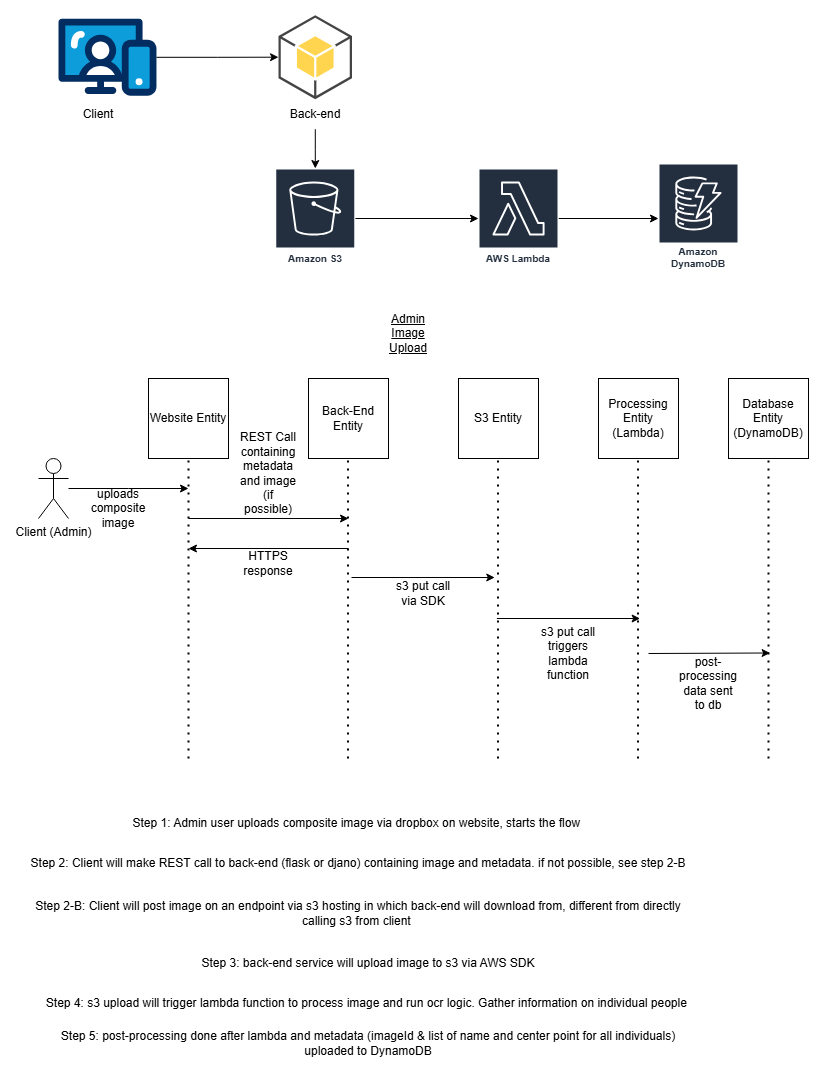
\includegraphics[width=0.7\textwidth]{ocr-arch_1.png}
\caption{Interface Software Architecture Design}
\label{FigUH}
\end{figure}

\section{Design of Communication Protocols}

\wss{NA}

\section{Timeline}

\wss{Schedule of tasks and who is responsible }
\wss{You can point to GitHub if this information is included there}

\subsection{Phase: Requirements Gathering and System Design}
\textbf{Dates:} Sept 23 – Oct 9 \\
\textbf{Tasks:}
\begin{itemize}
  \item Define functional and nonfunctional requirements
  \item Create high-level system architecture
\end{itemize}
\textbf{Responsible:}
\begin{itemize}
  \item All team members collaboratively
  \item Project Lead oversees progress
\end{itemize}


\subsection{Phase: Front-End and Back-End Development}
\textbf{Dates:} Oct 9 – Nov 22 \\
\textbf{Tasks:}
\begin{itemize}
  \item Develop front-end interface using React
  \item Implement back-end logic for data processing and storage
  \item Integrate APIs for OCR and composite data retrieval
\end{itemize}
\textbf{Responsible:}
\begin{itemize}
  \item Front-End: Willie, Henushan
  \item Back-End: Zahin, Wajdan, Henushan, Hammad
\end{itemize}

\subsection{Phase: Proof of Concept and Testing}
\textbf{Dates:} Nov 22 – Feb 3 \\
\textbf{Tasks:}
\begin{itemize}
  \item Deploy proof-of-concept prototype
  \item Perform unit, integration, and usability testing
  \item Address security and privacy compliance
\end{itemize}
\textbf{Responsible:}
\begin{itemize}
  \item Testing Lead: Hammad
  \item All members participate in debugging and verification
\end{itemize}

\subsection{Phase: Final Deployment and Demonstrations}
\textbf{Dates:} Feb 3 – Mar 30 \\
\textbf{Tasks:}
\begin{itemize}
  \item Complete final system deployment on McMaster servers
  \item Conduct usability testing and refine interface
  \item Prepare for final demonstration and Expo presentation
\end{itemize}
\textbf{Responsible:}
\begin{itemize}
  \item All members
  \item Final Presentation Lead: Willie
\end{itemize}

\subsection{Phase: Post-Deployment Support and Documentation}
\textbf{Dates:} Mar 30 – Apr 2 \\
\textbf{Tasks:}
\begin{itemize}
  \item Ensure system maintenance procedures are documented
  \item Provide user and administrator guides
\end{itemize}
\textbf{Responsible:}
\begin{itemize}
  \item Zahin, Hammad
\end{itemize}

\subsection{Task Tracking}
\textbf{Description:} Real-time task management and updates \\
\textbf{GitHub Repository:} \url{https://github.com/PaisWillie/Digital-Composite}

\bibliographystyle {plainnat}
\bibliography{../../../refs/References}

\newpage{}

\end{document}